%----------------------------------------------------------------------------------------
%	PACKAGES AND OTHER DOCUMENT CONFIGURATIONS
%----------------------------------------------------------------------------------------
\documentclass[paper=a4, fontsize=11pt]{scrartcl} % A4 paper and 11pt font size
\usepackage[T1]{fontenc} % Use 8-bit encoding that has 256 glyphs
\usepackage{fourier} % Use the Adobe Utopia font for the document - comment this line to return to the LaTeX default
\usepackage[english]{babel} % English language/hyphenation
\usepackage{amsmath,amsfonts,amsthm} % Math packages
\usepackage{lipsum} % Used for inserting dummy 'Lorem ipsum' text into the template
\usepackage{sectsty} % Allows customizing section commands
\allsectionsfont{\centering \normalfont\scshape} % Make all sections centered, the default font and small caps
\usepackage{fancyhdr} % Custom headers and footers
\usepackage[]{mcode}
\usepackage{amsmath}
\usepackage{graphics}
\usepackage{graphicx}

\pagestyle{fancyplain} % Makes all pages in the document conform to the custom headers and footers
\fancyhead{} % No page header - if you want one, create it in the same way as the footers below
\fancyfoot[L]{} % Empty left footer
\fancyfoot[C]{} % Empty center footer
\fancyfoot[R]{\thepage} % Page numbering for right footer
\renewcommand{\headrulewidth}{0pt} % Remove header underlines
\renewcommand{\footrulewidth}{0pt} % Remove footer underlines
\setlength{\headheight}{13.6pt} % Customize the height of the header

\numberwithin{equation}{section} % Number equations within sections (i.e. 1.1, 1.2, 2.1, 2.2 instead of 1, 2, 3, 4)
\numberwithin{figure}{section} % Number figures within sections (i.e. 1.1, 1.2, 2.1, 2.2 instead of 1, 2, 3, 4)
\numberwithin{table}{section} % Number tables within sections (i.e. 1.1, 1.2, 2.1, 2.2 instead of 1, 2, 3, 4)

\setlength\parindent{0pt} % Removes all indentation from paragraphs - comment this line for an assignment with lots of text

%----------------------------------------------------------------------------------------
%	TITLE SECTION
%----------------------------------------------------------------------------------------

\newcommand{\horrule}[1]{\rule{\linewidth}{#1}} % Create horizontal rule command with 1 argument of height

\title{	
\normalfont \normalsize 
\horrule{0.5pt} \\[0.4cm] % Thin top horizontal rule
\huge ECE 532 Homework 4: The SVD \\ % The assignment title
\horrule{2pt} \\[0.5cm] % Thick bottom horizontal rule
}

\author{Qihong Lu} % Your name
\date{\normalsize\today} % Today's date or a custom date

\begin{document}

\maketitle % Print the title

%----------------------------------------------------------------------------------------
%	PROBLEM 1
%----------------------------------------------------------------------------------------

\section*{Question1}
\textbf{A new user rated 25 our of 100 jokes. Use the first 20 rows of the data matrix predict her ratings for the rest of jokes. Compare your predictions to her complete set of ratings, contained in the vector trueb. Her actual favorite joke was number 29. Does it seem like your predictor is working well?}\\

We have a new user who rated 25 jokes, and we wish to predict her rating about the remaining 75 jokes, based on 20 old users, who rated all 100 jokes. \\

For the 25 jokes rated by the new users, we also have their ratings provided by 20 old users. So I used 20 users' rating about that 25 jokes as the matrix A, and the 25 joke's rating provided by the new user as y to computing the weights: 
$$ w = (A^T A)^{-1} A^T y $$
where $ A \in \mathbb{R}^{25x20}$ and $ y \in \mathbb{R}^{25x1}$, so the resulting weight is $w \in \mathbb{R}^{20x1}$ \\

Then the predicted rating for all 100 jokes is given by
$$
\text{prediction} = X w
$$ 
Where X is the 100 by 20 matrix that encode 20 users ratings about 100 jokes. \\

To evaluate the performance, I define the error as the following: 
$$\text{error} = \text{prediction} - \text{trueb}$$


\newpage
Here, I plotted the prediction errors for the 25 jokes rated by the new user on the left, and prediction errors for the 75 unrated jokes on the right panel. Prediction error of zero corresponds to perfect prediction. 

\begin{center}
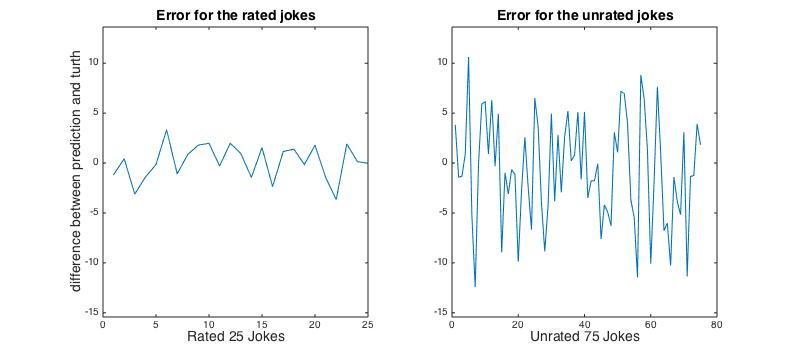
\includegraphics[scale=.6]{1_error.jpg}
\end{center}

The 25 jokes on rated by the user can be viewed as the training set for this problem. Note that the error for the training set is actually non-trivial. Moreover, the prediction error for the 75 unrated jokes is quite large. \\

I also computed the mean error as the following: 

$$
\text{meanError} = mean|error|
$$
where error is a vector that encodes the prediction error for all jokes. \\

The mean error for the 25 rated jokes is 1.4209. \\
The mean error for the 75 unrated jokes is 4.3814. \\

Moreover, according to the prediction, the new user's favoriate joke is joke 49, which is wrong. \\

In conclusion, the performance is not good. 


\newpage
Here is my matlab code: 
\begin{lstlisting}
%% Predict user ratings based on others
%% load the data matrix
clear all; clc; close all; 
% Each row is a joke, we have 100 jokes.  
% Each column is a user. We have 7200 users 
% Each of the users rated the quality of each joke on a scale of [?10, 10].
load('jesterdata.mat')
% load the partial data for the new user 
% b is the partial rating, the user rated x out of 100 jokes
load('newuser.mat')

%% read constant 
RATING.max = 10;
RATING.min = -10;
[numJokes, numUsers] = size(X);
% check the information provided 
ratedJokesIdx = (logical(b >= RATING.min) & logical(b <= RATING.max)); 
numRatedJokes = sum(ratedJokesIdx);
% select the first 20 columns 
Xsubset = X(:,1:20);

%% analysis 
% fit least square 
A = Xsubset(ratedJokesIdx,:);
y = b(ratedJokesIdx);
weights = inv(A'* A) * A' * y;

% compare to the truth 
prediction = Xsubset * weights;
testerror = prediction - trueb;

% plot the test error 
subplot(1,2,1)
plot(testerror(ratedJokesIdx))
ylim([min(testerror)-3 max(testerror)+3])
title('Error for the rated jokes', 'fontsize', 14)
ylabel('difference between prediction and turth', 'fontsize', 14)
xlabel('Rated 25 Jokes', 'fontsize', 14)
subplot(1,2,2)
plot(testerror(~ratedJokesIdx))
ylim([min(testerror)-3 max(testerror)+3])
title('Error for the unrated jokes', 'fontsize', 14)
xlabel('Unrated 75 Jokes', 'fontsize', 14)
% mean test error 
mean(abs(testerror(ratedJokesIdx)))
mean(abs(testerror(~ratedJokesIdx)))
% predict favoriate joke
find(prediction == max(prediction))
\end{lstlisting}
%----------------------------------------------------------------------------------------
%	PROBLEM 2
%----------------------------------------------------------------------------------------
\newpage
\section*{Question2}
\textbf{Repeat the prediction problem above, but this time use the entire X matrix. Note that now the problem is underdetermined. Explain how you will solve this prediction problem and apply it to the data. Does it seem like your predictor is working? How does it compare to the first method based on only 20 users?}\\ 


We still have a new user who rated 25 jokes, and we wish to predicther rating about the remaining 75 jokes.  Now the full matrix is avaliable, so we can base our prediction on 7200 old users who rated all 100 jokes. \\

If we want to solve the weight using the idea in question 1, we get: 
$$ w = (A^T A)^{-1} A^T y $$
but $ A \in \mathbb{R}^{25x7200}$, which means $A^TA$ is rank deficient and we cannot solve for it. Therefore, I applied the L-2 regularization and solve for the following: 
$$ w = (A^T A + \lambda I)^{-1} A^T y $$

I tried the following lambda values of 0.1, 0.2, 0.3, ..., 1. Although the errors on the 25 rated jokes are different, the errors on the 75 unrated jokes are all very close to 2.8391. When I plot the prediction errors for the 75 unrated jokes, the erros lines overlap with each other, illustrated below. 

\begin{center}
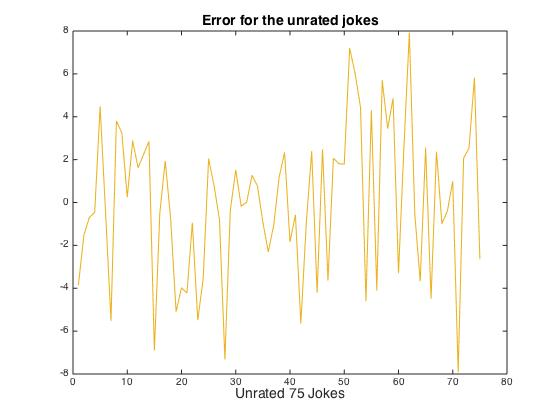
\includegraphics[scale=.6]{2_error.jpg}
\end{center}

Since the error on the hold out jokes is 2.8391, this is better than question1, when I just used the data from 20 users. However, the performance is still unsatisfying. 

\newpage
Here is the matlab code for question 2. 
\begin{lstlisting}
%% Predict user ratings based on others
%% load the data matrix
clear all; clc; close all; 
% Each row is a joke, we have 100 jokes.  
% Each column is a user. We have 7200 users 
% Each of the users rated the quality of each joke on a scale of [?10, 10].
load('jesterdata.mat')
% load the partial data for the new user 
% b is the partial rating, the user rated x out of 100 jokes
load('newuser.mat')

%% read constant 
RATING.max = 10;
RATING.min = -10;
[numJokes, numUsers] = size(X);
% check the information provided 
ratedJokesIdx = (logical(b >= RATING.min) & logical(b <= RATING.max)); 
numRatedJokes = sum(ratedJokesIdx);

%% analysis 
% fit least square 
A = X(ratedJokesIdx,:);
y = b(ratedJokesIdx);
I = eye(numUsers);

% choose lambda, preallocate for errors
lambdas = 1e-1 :1e-1: 1;
prediction = nan(numJokes, length(lambdas));
% loop over all lambdas
for i = 1 : length(lambdas)
    lambda = lambdas(i);
    weights = inv(A'* A + lambda * I) * A' * y;
    % compute the prediction 
    prediction(:,i) = X * weights;
end
errors = bsxfun(@minus, prediction, trueb);

%% plot the test error 
% plot the test error 
plot(errors(~ratedJokesIdx,:))
title('Error for the unrated jokes', 'fontsize', 14)
xlabel('Unrated 75 Jokes', 'fontsize', 14)
% compute the mean absolute errors
mean(abs(errors(~ratedJokesIdx,:)))
% find the predicted best joke
for lambdaIdx = 1:10; 
    find(prediction(:,lambdaIdx) == max(prediction(:,lambdaIdx)));
end
\end{lstlisting}
%----------------------------------------------------------------------------------------
%	PROBLEM 3
%----------------------------------------------------------------------------------------
\newpage
\section*{Question3}
\textbf{Propose a method for finding one other user that seems to give the best predictions for the new users. How well does this approach perform? Now try to find the best two users to predict the new user.} \\ 


I chose the user associated with the largest weight magnitude when fitting ridge regression model. The 2503th user has the largest absolute weight $(-0.0025)$. The 500th user has the second largest absolute weight value $(0.0024)$.\\

After choosing these two users, combining their ratings give me a 100 by 2 matrix. Now, I am no long in the underdetermined case, so I can repeat the procedure conducted in question 1. \\

After fitting the least square, the average prediction error for the 75 rated jokes is 2.5446. And the average prediction error for the 25 unrated jokes is  1.6751. \\

Since the error on the holdout jokes is lower than both previous methods (used in question 1 and 2). This method seems to be a surprisingly good idea. 


\newpage
\begin{lstlisting}
%% Predict user ratings based on others
%% load the data matrix
clear all; clc; close all;
% Each row is a joke, we have 100 jokes.
% Each column is a user. We have 7200 users
% Each of the users rated the quality of each joke on a scale of [?10, 10].
load('jesterdata.mat')
% load the partial data for the new user
% b is the partial rating, the user rated x out of 100 jokes
load('newuser.mat')

%% read constant
RATING.max = 10;
RATING.min = -10;
[numJokes, numUsers] = size(X);

% check the information provided
ratedJokesIdx = (logical(b >= RATING.min) & logical(b <= RATING.max));
numRatedJokes = sum(ratedJokesIdx);

%% fit the model
A = X(ratedJokesIdx,:);
y = b(ratedJokesIdx);
I = eye(numUsers);
lambda = 1;
% fit ridge regression
weights = inv(A'* A + lambda * I) * A' * y;
% compute the prediction
prediction = X * weights;

%% find indices for the largest and second largest weights 
idx.largest1 = find(abs(weights) == max(abs(weights)));   % max 
idx.largest2 = find(abs(weights) == max(weights(abs(weights) < max(abs(weights)))));  % 2nd largest 
% get the data matrix 
Anew = [A(:,idx.largest1) A(:,idx.largest2)];
Xnew = [X(:,idx.largest1) X(:,idx.largest2)];
% figure out the weights
weightsNew = inv(Anew' * Anew) * Anew' * y;
% generate the prediction
prediction = Xnew * weightsNew;
% compute the error 
error = prediction - trueb;

%% show the error 
% plot the test error 
subplot(1,2,1)
plot(error(ratedJokesIdx))
title('Error for the rated jokes', 'fontsize', 14)
ylabel('difference between prediction and turth', 'fontsize', 14)
xlabel('Rated 25 Jokes', 'fontsize', 14)
subplot(1,2,2)
plot(error(~ratedJokesIdx))
title('Error for the unrated jokes', 'fontsize', 14)
xlabel('Unrated 75 Jokes', 'fontsize', 14)

% compute mean error
mean(error(ratedJokesIdx))
mean(error(~ratedJokesIdx))
\end{lstlisting}

%----------------------------------------------------------------------------------------
%	PROBLEM 4
%----------------------------------------------------------------------------------------
\newpage
\section*{Question4}
\textbf{Use the Matlab function svd with the economy size option to compute the SVD of $X = U \Sigma V^T $. Plot the sprectrum of X. What is the rank of X? How many dimensions seem important? What does this tell us about the jokes and users?}\\

Here's the plot for the singular values of X, ordered by magnitude.
\begin{center}
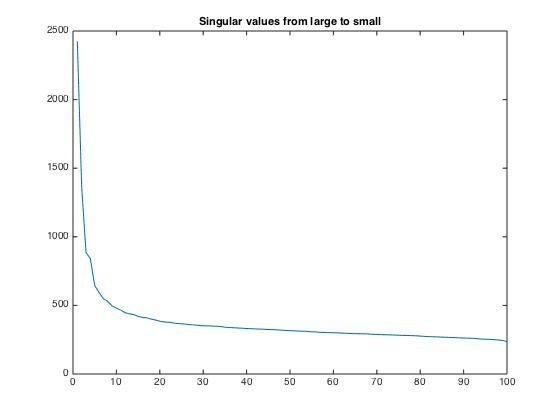
\includegraphics[scale=.6]{4_sv.jpg}
\end{center}

First of all, non of the singular value is approximately zero. It could be that the data for jokes are quite complex, or the noise in this data is is too big. \\

Also, it seems that the first 10 singular values are substantially larger than the rest, which indicates the first 10 dimensions are really important. Although the joke rating data has rank 100, it seems that the first 10 pinciple components should be sufficient to account for most of variance of this data set. This tells us that the joke rating data approximately live in a 10 dimensional subspace. \\

In terms of the jokes, one can argue that the first 10 pinciple components captured the 10 most "representative" jokes, based on the users rating. In particular, the rest of jokes can be approximated by the linear combination of these 10 jokes fairly well. \\

In terms of the users, the first 10 pinciple components captured the 10 most "representative" users, based on their ratings of the jokes. Specifically, the rest of the users can be approximated by the linear combination of these 10 users fairly well. 

\newpage
Here's the matlab code for question 4. 
\begin{lstlisting}
%% Predict user ratings based on others
%% load the data matrix
clear all; clc; close all; 
% Each row is a joke, we have 100 jokes.  
% Each column is a user. We have 7200 users 
% Each of the users rated the quality of each joke on a scale of [?10, 10].
load('jesterdata.mat')
% load the partial data for the new user 
% b is the partial rating, the user rated x out of 100 jokes
load('newuser.mat')

%% read constant 
RATING.max = 10;
RATING.min = -10;
[numJokes, numUsers] = size(X);

% check the information provided 
% rateJokesIdx = (logical(b >= RATING.min) & logical(b <= RATING.max)); 
% numRatedJokes = sum(rateJokesIdx);

% compute the singular value decomposition with the first 20 rows
[U,S,V] = svd(X, 'econ');

%% plot spec(X)
plot(diag(S));
title('Singular values from large to small')
rank(X)
\end{lstlisting}

%----------------------------------------------------------------------------------------
%	PROBLEM 5
%----------------------------------------------------------------------------------------
\newpage
\section*{Question5}
\textbf{Visualize the dataset by projecting the columns and rows on to the first three principle component directions. Discuss the structure of the projections and what it might tell us about the jokes and users.}\\
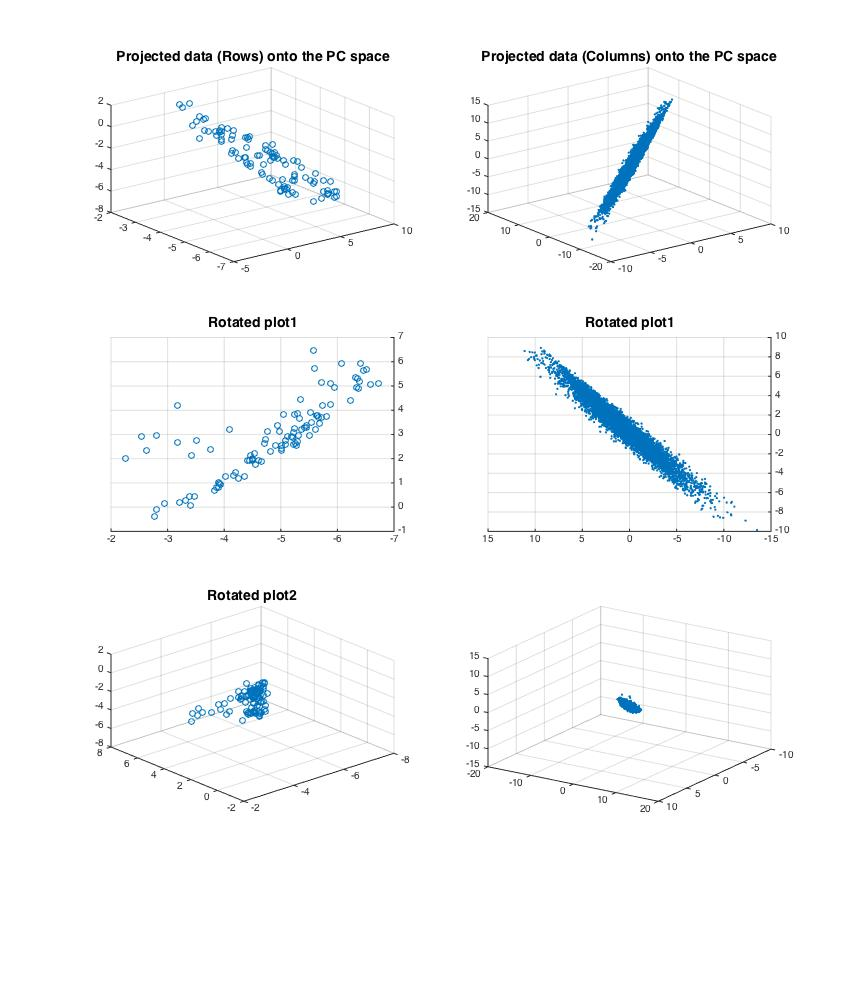
\includegraphics[scale=.5]{5_scat.jpg}\\

On the left, each point represents a joke and the features are the users. On the right, each point is a user, and the features are the jokes. They are connected by the ratings. \\

For both plots, it we approximate it by a ellipse, it is quite thin. This implies that the first pinciple component is significantly larger than the second and the third. \\

Because the first principle direction captures so much variance in the data set, it means that it there is one dimension that is particularly important for how user rate the jokes and it is possible to find a most "representative" user that captures the behavior of most of the users. 

\newpage
Here's the matlab code for question 5
\begin{lstlisting}
%% load the data matrix
clear all; clc; close all; 
load('jesterdata.mat')
%% compute the SVD
[U,S,V] = svd(X, 'econ');
%% dimensionality reduction 
subspaceDim = 3; 
% project rows
pcsV = V(:,1:subspaceDim);
projMatV = pcsV*inv(pcsV'*pcsV)*pcsV';
projectedX_v = X * projMatV;
XpV = projectedX_v(:,1:subspaceDim);
% project columns
pcsU = U(:,1:subspaceDim);
projMatU = pcsU*inv(pcsU'*pcsU)*pcsU';
projectedX_u = X' * projMatU;
XpU = projectedX_u(:,1:subspaceDim);

%% plot rows 
subplot(3,2,1)
scatter3(XpV(:,1),XpV(:,2),XpV(:,3))
title('Projected data (Rows) onto the PC space', 'fontsize', 14)
subplot(3,2,3)
scatter3(XpV(:,1),XpV(:,2),XpV(:,3))
title('Rotated plot1', 'fontsize', 14)
subplot(3,2,5)
scatter3(XpV(:,1),XpV(:,2),XpV(:,3))
title('Rotated plot2', 'fontsize', 14)

%% plot columns 
subplot(3,2,2)
scatter3(XpU(:,1),XpU(:,2),XpU(:,3), '.')
title('Projected data (Columns) onto the PC space', 'fontsize', 14)
subplot(3,2,4)
scatter3(XpU(:,1),XpU(:,2),XpU(:,3), '.')
title('Rotated plot1', 'fontsize', 14)
subplot(3,2,6)
scatter3(XpU(:,1),XpU(:,2),XpU(:,3), '.')
\end{lstlisting}

%----------------------------------------------------------------------------------------
%	PROBLEM 6
%----------------------------------------------------------------------------------------
\newpage
\section*{Question6}
\textbf{One easy way to compute the first principle component for large datasets like this is the so-called power method. Explain the power method and why it works. Write your own code to implement the power method in Matlab and use it to compute the first column of U and V in the SVD of X. Does it produce the same result as Matlab's built-in svd function?}\\


Yes, it can approximate the first left and right singular vector and the first singular value, which can be verified by the matlab svd function. I chose a random real valued vector initially (by randn), and apply the power method for each iteration. Here's an visualization of the error of my approximation over iterations. The error is defined as the 2 norm of the difference between the absolute value of the approximating vector and the truth first singular vector (computed by svd). As you can see, after 6 iterations, the error is already approximately zero. 

\begin{center}
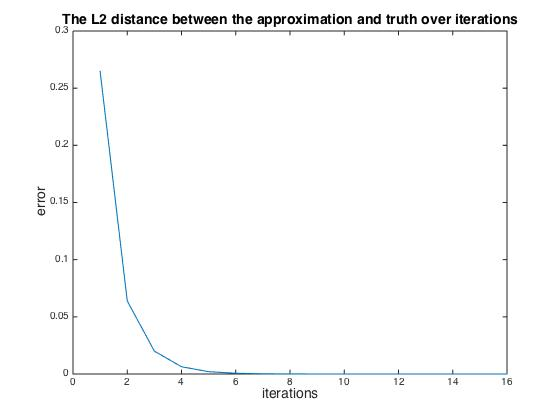
\includegraphics[scale=.5]{6_err.jpg}
\end{center}


Why it works? 

The power method is approximating the eigenvector associated with the largest eigenvalue. To compute the first right singular vector for a given matrix $X$, I just need to plug in $X^TX$, because the eigenvector associated with the largest eigenvalue of $X^TX$ is the first right singular vector of $X$, and the largest eigenvalue of $X^TX$ is the square of the largest singular value of $X$. This can be seen by the following reaonsing: 
$$
X = U \Sigma V^T \text{(singular value decomposition)}
$$
$$
X^TX = V \Sigma^T U^T U \Sigma V^T = V \Sigma^2 V^T \text{(This is in the form of eigen decompostion)}
$$
(The argument for $XX^T$ is symmertic)

\newpage

Here's the matlab code for question 6: 
\begin{lstlisting}
%% Predict user ratings based on others
%% load the data matrix
clear all; clc; close all; 
load('jesterdata.mat')
[m,n] = size(X);
[U,S,V] = svd(X);

%% use the power method to approximate the first right singular vector
i = 0; 
v1 = randn(n,1);
while i < 50
    % perform the power iteration
    v1 = X'*X * v1 / norm(X'*X * v1,2);
    i = i+1;
    % record the error, stop when the error is small 
    error(i) = norm(abs(v1) - abs(V(:,1)));
    if error(i) < 1e-8
        break;
    end
end

%% get 1st L/R singular vectors and singular value
% now v1 is the 1st right singular vector
% sigma1 is the first singular value
sigma1 = norm(X * v1,2);
% u1 is the 1st left singular vector
u1 = X * v1 / sigma1;

%% visualize the performance
plot(error)
tt = sprintf('The L2 distance between the approximation and truth over iterations');
title(tt, 'fontsize', 14)
ylabel('error', 'fontsize', 14)
xlabel('iterations', 'fontsize', 14)
\end{lstlisting}

%----------------------------------------------------------------------------------------
%	PROBLEM 7
%----------------------------------------------------------------------------------------
\newpage
\section*{Question7}
\textbf{The power method is based on an initial starting vector. Give one example of a starting vector for which the power method will fail to find the first left and right singular vectors in this problem.}\\

If I initialize the approximation vector $b_0$ as the zero vector, this method is not going to work. Because if the initial vector is all zero vector, the denominator $||Ab_0|| = 0 $. \\

I used my code to verify this. When I initalize the approximating vector as the zero vector, it outputs a "NA" vector at the end. 

\end{document}